\documentclass{article}

\usepackage[final]{nips_2016}

\usepackage[utf8]{inputenc} % allow utf-8 input
\usepackage[T1]{fontenc}    % use 8-bit T1 fonts
\usepackage{url}            % simple URL typesetting
\usepackage{booktabs}       % professional-quality tables
\usepackage{amsfonts}       % blackboard math symbols
\usepackage{nicefrac}       % compact symbols for 1/2, etc.
\usepackage{microtype}      % microtypography
\usepackage{graphicx}
\usepackage{amssymb}
\usepackage{amsmath}
\usepackage[titletoc,toc,page]{appendix}
\usepackage{verbatim}
\usepackage[colorlinks=true,citecolor=blue]{hyperref}

\bibliographystyle{alpha}

\newtheorem{theorem}{Theorem}
\newtheorem{property}{Property}

% use this to signal places where it'd be nice to cite something
\newcommand{\needcite}{${}^{\text{\color{red}[citation needed]}}$}

\title{Semi-Supervised Learning on Graphs \\
for Inverse Reinforcement Learning}

\author{
Élie Michel\\
Department of Computer Science\\
École normale supérieure\\
Paris, France\\
\texttt{elie.michel@ens.fr}
\And
Charles Reizine\\
Department of Computer Science\\
École Nationale des Ponts et Chaussées\\
Paris, France\\
\texttt{charles.reizine@eleves.enpc.fr}
}

% Not cited:
%\cite{Littman94} -> about RL

\begin{document}

\maketitle

\begin{abstract}
This paper starts with a short review on \emph{Inverse Reinforcement Learning} (IRL) and on the interest there is in coupling IRL to \emph{Semi Supervised Learning} (SSL) using graphs. The purpose of IRL is to use  \emph{trajectories} (i.e. sequence of successing states) generated by a set of expert supposedly behaving according to a reward function R, to retrieve this reward function. In this review, we focused on the setup where it's easy to observe large set of \emph{trajectories}, but where only a few of them can be labelled. After introducing the general setup of IRL and it limitations, we presented the general purpose and interest of the use of graphs for SSL. Finally, we discussed the interest of associating IRL to graphs SSL and present some of the apparent limitations of this process. The core of our project consisted in obtaining a graph SSL problem from \emph{Markov Decision Process} (MDP) trajectories. We also discussed the matter of using bad examples for improving IRL results'.
\end{abstract}

\section{Introduction}

The goal of \emph{Inverse Reinforcement Learning} (IRL) is to learn the reward function in a \emph{Markov Decision Process} (MDP) from the demonstrations of expert agents. It has many applications \cite{Kaelbling96} but, as many ML problems, it often suffers from lack of training data as for instance pointed out in \cite{Vasquez14}. \emph{Semi-Supervised Learning} (SSL) is a typical approach to tackle this issue. In this work, we explore the application of SSL methods to the class of IRL problems.
\paragraph{}
In IRL, we suppose that we possess a set of trajectories generated by experts abiding by an optimal strategy. Our purpose would be to use SSL approaches to differenciate positive and negative trajectories. Thanks to this process, we could use larger, partially labeled, set of trajectories to perform IRL. The use of unlabeled trajectories represents a true challenge because SSL methods are based on the notion of similarity which is hard to design on such complex objects.
%% Je te laisse le paragraphe descriptif pour être sûr qu'il y a tout ce que tu cherchais dans ce que j'écris 
\paragraph{FIXME} % entre pas dans les détails, c'est vraiment l'intro de l'intro, mentionne juste tous les points (et répond aux questions, les laisse pas tel quel ^^ les questions rhétoriques c'est pas ouf dans un article scientifique)
Write a little § about:
Why is it interesting to focus on this?
Which are the challenges?

 - IRL is ill-posed

 - pb of measure of similarity to apply ssl
 
 - we use ssl to differentiate positive from negative examples

 - apply ssl to objects which are trajectories -> similarity hard to design

% Annonce du plan
\paragraph{}
We first review the challenges of IRL in Section~\ref{sec:irl} on one hand and SSL in Section~\ref{sec:ssl} in the other hand. In Section~\ref{sec:combine}, we present the pipeline in which we combine both problems and the main issues we then face. Then Section~\ref{sec:results} presents our application cases and elements of results. Finally, Section~\ref{sec:limitations} reviews the main limitations of our approach suggest some future work.


%%%%%%%%%%%%%%%%%%%%%%%%%%%%%%%%%%%%%%%%%%%%%%%%%%%%%%%%%%%%%%%%%%%%%%%%%%%%%%%
\section{Inverse Reinforcement Learning \label{sec:irl}}

%------------------------------------------------------------------------------
\subsection{Introduction to Reinforcement Learning}

\paragraph{}
The general idea of Reinforcement Learning (RL) \cite{Sutton98} is to determine the optimal action policy of a given agent so that it maximizes a \emph{reward} (also called \emph{reinforcement function}) $R$ provided by its interaction with an environment (see Figure~\ref{fig:rl}).

\begin{figure}
\begin{center}
  \makebox[\textwidth]{
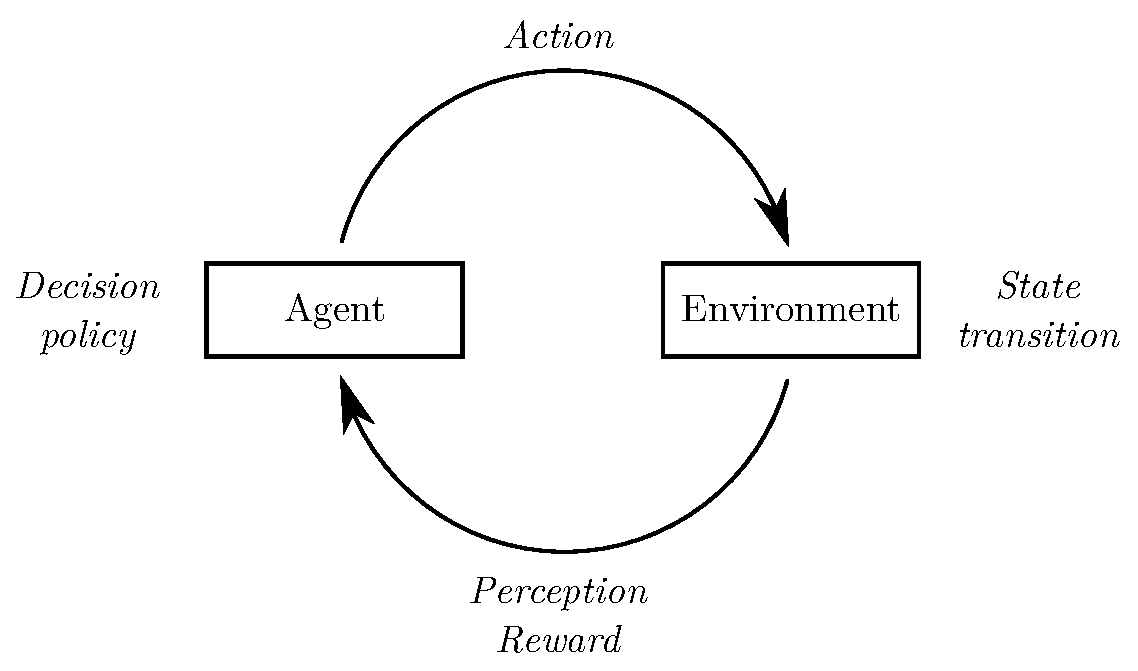
\includegraphics[width=0.4\paperwidth]{rl.eps}
}
\end{center}
\caption{Traditional scheme of Reinforcement Learning. The usual RL task consists in determining a decision policy while the task of IRL is to find the reward function. Other problems are sometimes studied, like infering the perception in cognitive science. \label{fig:rl}}
\end{figure}

\subsubsection{Formalization of the setup}

This setup is formalized around the model of \emph{Markov Decision Process} (MDP), often assigned to Bellman and his work in Dynamic Programing (already mentioned in \cite{Bellman57}), and used by \cite{Watkins89} as a basis to develop the main RL algorithms such as Q-Learning. A finite MDP is defined as a tuple $(S,A,\{P_{sa}\},\gamma,R)$, where

\begin{itemize}
    \item $S$ is a finite set of $N$ \emph{states}
    \item $A=\{a_1,...,a_k\}$ is a set of $k$ \emph{actions}
    \item $P_{sa}$ are the state \emph{transition probabilities} upon taking action $a$ in state $s$
    \item $\gamma$ is the \emph{discount factor} tunning the long term influence of previous reward
    \item $R$ is the \emph{reward function} (bounded)
\end{itemize}

A \emph{policy} is a map $S \rightarrow A$, potentially probabilistic. Its value is defined as the expected \emph{return} of the agent when sampling actions following this policy:

\[
V^{\pi} = \mathbb E[r_0 + \gamma r_1 + \gamma^2 r_2 + \dots|\pi]
\]

where $r_t$ is the reward received at time $t$.

\paragraph{NB} We consider stationary policies, so this model represents jointly as state both environement-related  states and agent's internal state like memory effects. The policy cannot track information about the trajectory beyond what the state space encodes.

\subsubsection{Missing Reward}

RL has been applied to a wide variety of problems ranging from robotics \cite{Kober13} to economics \cite{Tesauro02} with impressive results, especially in the field of games \cite{Silver16}. But in many real life problems, the main bottleneck to the application of RL is that the hypothesis of a perfectly known reward function $R$ is not satisfied. For instance, the exact reward maximized during car driving \cite{Shalev16} or human walk \cite{Morimoto04} remains unknown.

%------------------------------------------------------------------------------
\subsection{Inverse problem}

Noticing this issue, \cite{Russell98} introduces the notion of Inverse Reinforcement Learning. Instead of looking for a policy given a reward, the algorithm is provided with a policy and asked to determine a reward function for which this policy is optimal. In other words, IRL is intended to build a reward that can explain the observed behavior of an agent.

\subsubsection{First formalization}

This problem has remained ill-posed for some time. A first attempt to formalized it is presented in \cite{Ng00}, which notice that the constraint of $\pi$ being optimal can be rewritten as in Property~\ref{prop:irl}.

\begin{property}
\label{prop:irl}
Let  $(S,A,P_{sa},\gamma,R)$ be a MDP where $S$ is a finite space and $\gamma \in (0,1)$. A policy $\pi$ is optimal if and only if, for all $a=a_{2},...,a_{k}$, the reward satisfies :

\[
(P_{\pi(s)} - P_a)(I - \gamma P_{\pi(s)})^{-1} R \succeq 0
\]
\end{property}

\subsubsection{Additional constraints}

\cite{Ng00} then leverage on this to write IRL as a linear program and apply it to a toy problem (5x5 grid world), but highlights that the problem misses some constraint for the trivial solution where the reward is constant not to be a valid output. Heuristic constraints making the reward more discriminative are explored, such as using reward shaping \cite{Ng99} or maximizing

\[
\sum _{s \in S}\left(Q^\pi(s, a_1) - \max_{a \in A \setminus a_1} Q^\pi(s,a)\right)
\]

\paragraph{}
In large or continuous state systems, the reward cannot be built for each state independently so it is modelized as a combination of hand written feature functions like in Figure~\ref{fig:features}, first linearly combined \cite{Abbeel04} and more recently with gaussian mixture of features \cite{Levine11}.

\begin{figure}
\begin{center}
  \makebox[\textwidth]{
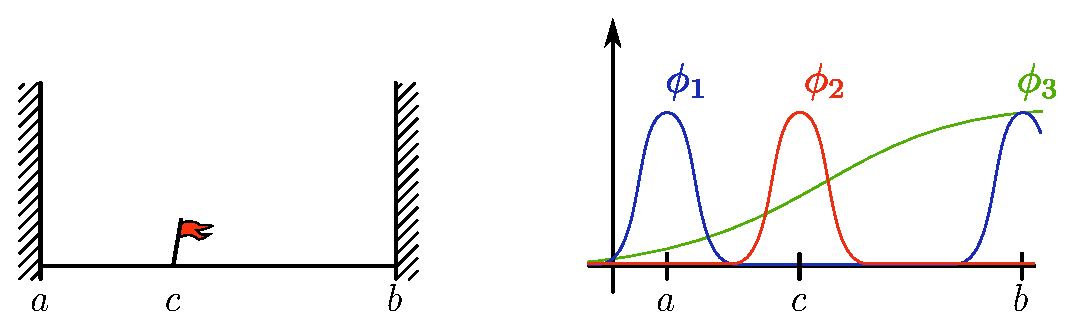
\includegraphics[width=0.5\paperwidth]{features.eps}
}
\end{center}
\caption{Example of feature functions. If our agent is a cart evolving in the continuous linear world of the left-hand side, the functions $\phi_i$ can be used as features to be combined to modelize $R$. Here the qualitative meaning of these hand-made function could be "be close to the walls" for $\phi_1$, "be close to the flag for $\phi_2$ and "be on the right-hand side" for $\phi_3$. \label{fig:features}}
\end{figure}

\subsubsection{Limitations of strict IRL}

\cite{Ng00} quickly notice that this approach scales up poorly to more complex problems that don't come with a full policy. It is particularly problematic for large or continuous state spaces for which it is virtually impossible to enumerate the policy for every state\footnote{unless the problem admits some analytic solution, which is barely never the case in actual applications}.

%------------------------------------------------------------------------------
\subsection{IRL from sampled trajectories}

\paragraph{}
The input is hence relaxed from knowing the whole optimal policy to knowing only a set of trajectories sampled using this trajectories. This matches a setup in which one can record from an expert agent (e.g. a human driver for autonomous driving problem) its sequence of actions given a situation, or many situations, but not explicit the full policy.

\paragraph{}
\cite{Ng00} already addresses this issue and more recent work mainly focus on this case.

\subsubsection{Exploration problem}
The main qualitative issue of using only sampled trajectories to determine $R$ is that it requires these trajectories to go at some point through each point of the state space.

\begin{figure}
\begin{center}
  \makebox[\textwidth]{
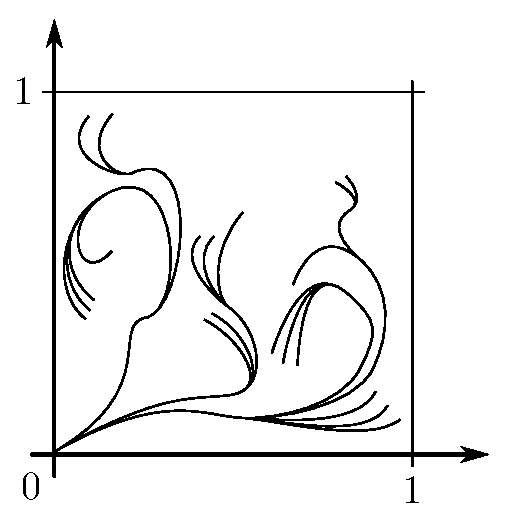
\includegraphics[width=0.3\paperwidth]{continuous-grid.eps}
}
\end{center}
\caption{Imaginary example of linear trajectories sampled in a continuous 2-dimensional state space showing that a vast majority of states are never visited in practice, hence the need for feature functions. \label{fig:continuous-grid}}
\end{figure}


\paragraph{}
So one would need either many trajectories or trajectories long enough with respect to the number of states. Not only it is not tractable in the case of large or continuous state spaces as illustrated in Figure~\ref{fig:continuous-grid}, but there is also no garanty that even among many trajectories one would go through each state.

\subsubsection{Reduction of dimensionality}
To tackle the problem of having too many states to explore, the dimensionality of the reward function is dramatically reduced by feature based approximations \cite{Abbeel04, Levine11} as in Figure~\ref{fig:features} where $R$ is a combination of a number of features small with respect to the number of training trajectories. Alternatively, or complementarily, one could use IRL to build $R$ only on an explored subset of the state space and then generalize using \cite{Finn17}.

\subsubsection{Negative examples}
Another way to augment the training data is to consider also \emph{negative examples}, i.e. examples of bad trajectories that a good policy should not follow (see Figure~\ref{fig:negpos}).


\begin{figure}
\begin{center}
  \makebox[\textwidth]{
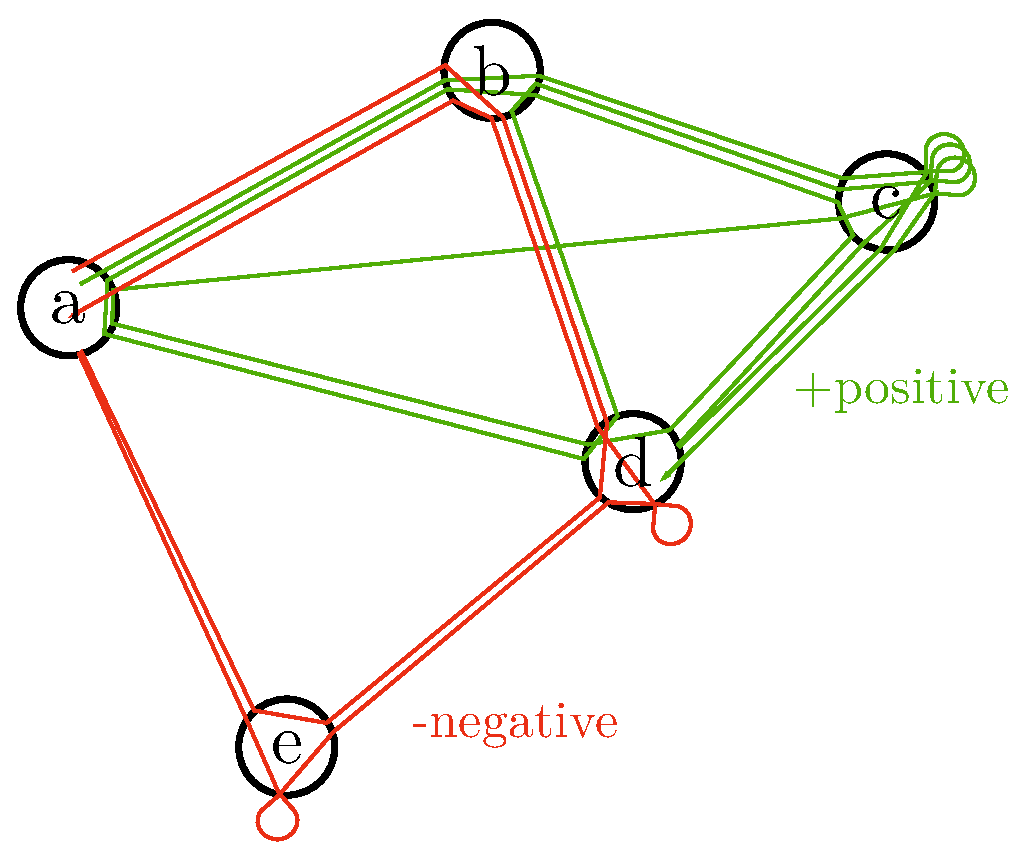
\includegraphics[width=0.3\paperwidth]{negpos.eps}
}
\end{center}
\caption{Example of two trajectories in a five states MDP with one labeled as positive and the other one labeled as negative. One can notice that some states like $c$ and $e$ are not reached at all by some trajectories. \label{fig:negpos}}
\end{figure}


\paragraph{}
As pointed out in \cite{Lee16}, which introduces a very interesting way of doing IRL with negative examples, this is a way to learn properly in regions of the state space with low reward which are thus rarely explored by positive examples.

\paragraph{}
This approach also has the advantage of invalidating the anoying trivial solutions of IRL such as constant reward and hence makes the problem better posed.


%%%%%%%%%%%%%%%%%%%%%%%%%%%%%%%%%%%%%%%%%%%%%%%%%%%%%%%%%%%%%%%%%%%%%%%%%%%%%%%
\section{Semi-Supervised Learning \label{sec:ssl}}

\paragraph{TODO} \emph{This whole section needs a refresh and citations.}

%------------------------------------------------------------------------------
\subsection{Semi-supervised learning in Graphs}

Semi-supervised learning is a class of supervised learning tasks and techniques that also make use of unlabeled data for training. This is useful when a large set of data is available but only a small amount of it has already been labeled.
The use of graphs for SSL is a transductive approach \cite{chapelle09} that has become widely used after \cite{Zhu03}.
The idea is to use the input data to build a graph and to use it to label each of the node. To construction of the graph is based on the notion of similarity between nodes. 

On some simple problems, the similarity can be built from the euclidian distance between the input vectors. Nonetheless, on more complex issues, similarities are harder to build. We will discuss the mater of building a relevant similarity for trajectories in the next section.

When similarities have been computed, the graph can be built and we can proceed to SSL (via hard or soft harmonic functions for instance \cite{doyle84}. This is why we will focus on the construction of a relevant similarity function for trajectories.

%%%%%%%%%%%%%%%%%%%%%%%%%%%%%%%%%%%%%%%%%%%%%%%%%%%%%%%%%%%%%%%%%%%%%%%%%%%%%%%
\section{Mixed pipeline of SSL for IRL problem \label{sec:combine}}

The need for SSL arises as soon as we switch from having only positive examples to having both positive and negative examples. While in the first case we do not need labeling in the sens that all samples have the same (positive) label, adding negative examples requires labeling, and so potentially human intervention.

\paragraph{}
While we could imagine more tied mix of SSL and IRL, we focus here on how to apply SSL to objects which are sampled trajectories whose only some of them are labeled (\emph{good} or \emph{bad}) and apply IRL in a second step on reconstructed labels (see Firgure~\ref{fig:pipeline}). This can be seen as a simplification of the task of estimating the return of a trajectory \needcite [is this done w/ DNNs sometimes?].

\begin{figure}
\begin{center}
  \makebox[\textwidth]{
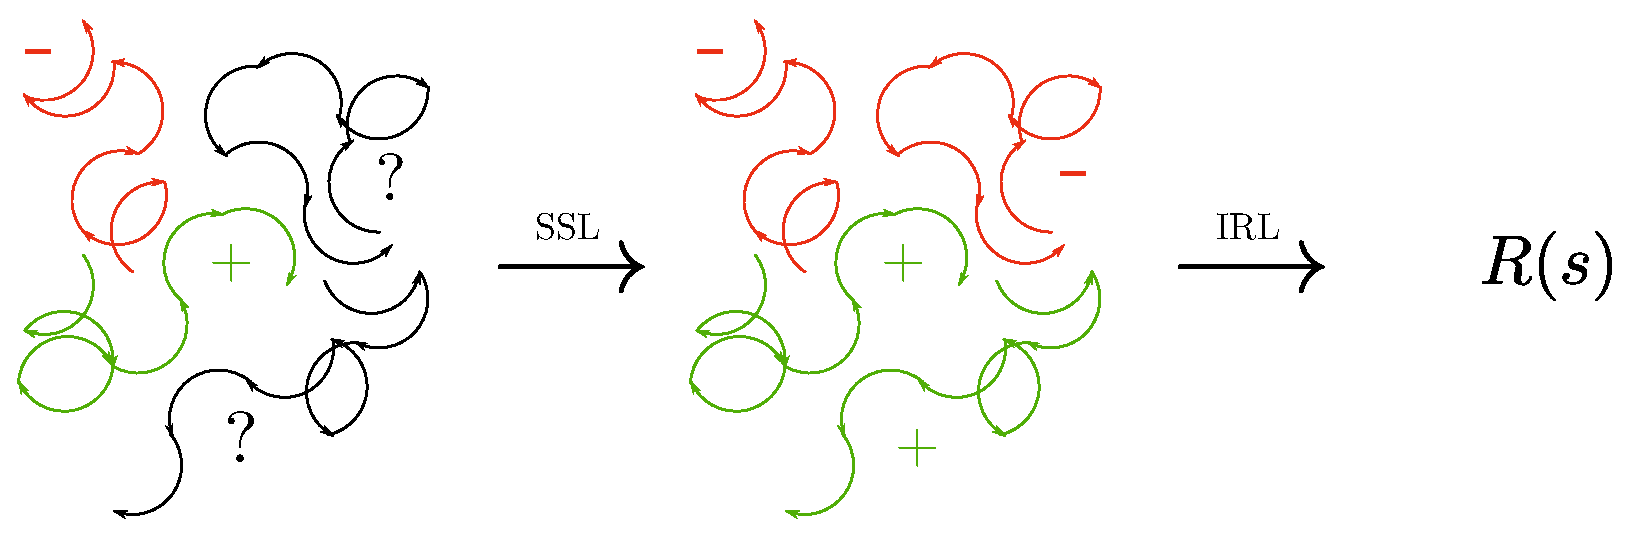
\includegraphics[width=0.6\paperwidth]{pipeline.eps}
}
\end{center}
\caption{Pipeline using SSL to label positive and negative trajectories for IRL\label{fig:pipeline}}
\end{figure}

\paragraph{}
The combination of SSL and IRL has been used in \cite{Valko12} in which the authors aim at improving the max margin classification learning over trajectories by augmenting the set of labeled trajectories with unlabeled trajectories. As well, in \cite{Audiffren15}, authors succed in improving MaxEnt-IRL algorithm thanks to the use of unsupervised trajectories.

\paragraph{}
Following another approach, \cite{Finn17} consider that the reward is known on a subset of the state space only and makes use of unlabeled MDPs in order to generalize it.

%------------------------------------------------------------------------------
\subsection{Trajectory Similarity}

At the core of SSL methods on graphs is the notion of similarity, which enables one to propagate labels from known points to unknown ones. While measuring similarity between fixed size feature vectors is quite straightforward, at least using euclidian distance as a first approximation, designing a measure of similarity between two trajectories is trickier.

\paragraph{}
We first introduce our measure of similarity in the case of single state setups, also called \emph{Multi-Arm Bandits} (MAB), and then generalize to multiple states.

\subsubsection{Similarities between Multi-Arm Bandits trajectories}

A good thing with MAB is that there is no notion of order in the sequence of actions chosen by a stationary policy. So we can focus on the \emph{histogram} of the trajectories only. Once normalized to harmonize the different lengths of sequences, what we obtain is exactly the empirical distribution of probability of drawing the different arms (see Figure~\ref{fig:hist}).

\begin{figure}
\begin{center}
\makebox[\textwidth]{
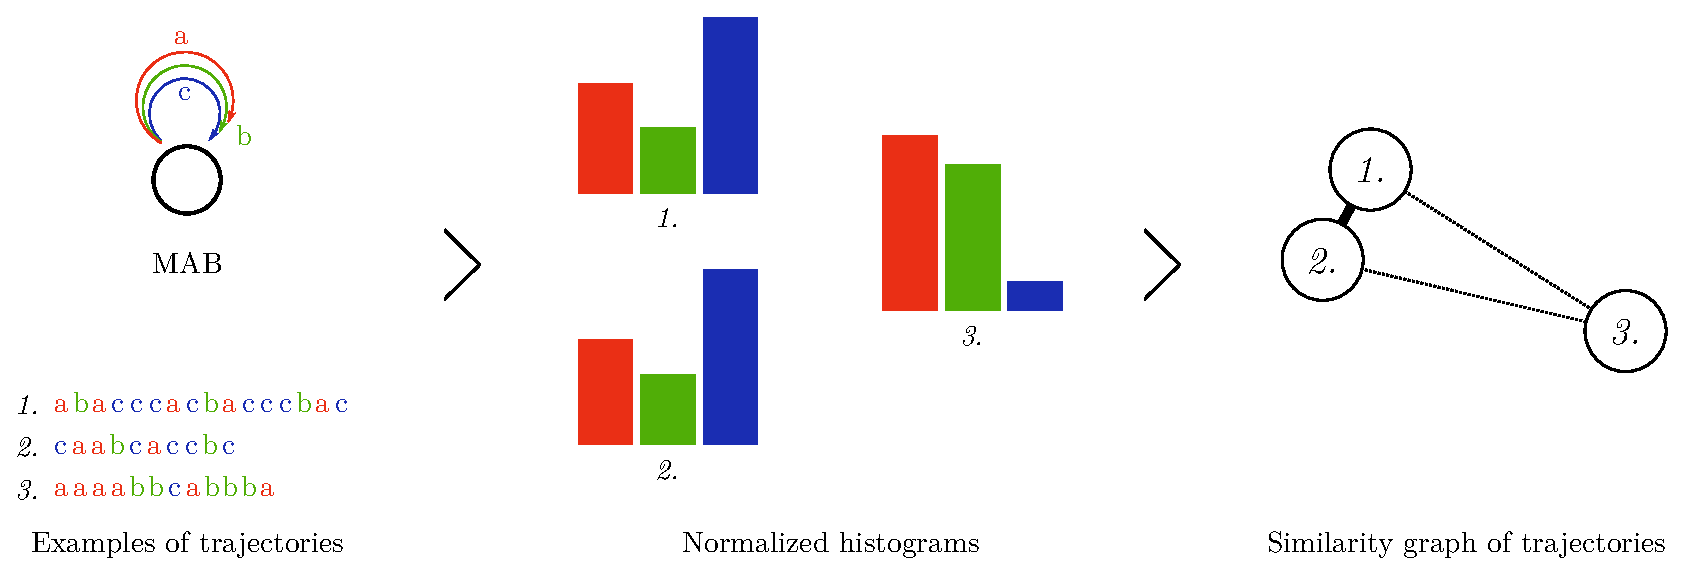
\includegraphics[width=0.6\paperwidth]{hist.eps}
}
\end{center}
\caption{Example of policy estimation from trajectories in MAB for similarity measure. Trajectories $1$ and $2$ are close while $3$ is further. \label{fig:hist}}
\end{figure}

\paragraph{}
We can then use traditional measures of similarity between distributions, such as (normalized) mutual information or (symmetrized) Kullback–Leibler divergence \cite{Kullback51}. We define the similarity between trajectories $T_1$ and $T_2$ as

\[
\text{similarity}(T_1, T_2) = \text{NMI}(\text{nhist}(T_1), \text{nhist}(T_2))
\]

where $\text{nhist}(T)$ is the normalized histogram of $T$.

\subsubsection{Generalization}

We then generalize this approach to multiple state MDPs. If a state is visited several times by the same trajectory, it is possible to estimate in the same way the policy at this state. We estimate the underlying matrix $P$ such that:

\[
\hat P_{a,s} = \mathbb P(\text{chosing action } a | \text{being in state } s)
\]

As for MABs, we can then compare two trajectories on a given state using a distribution similarity measure. We then sum this measure over all the states since these are independent properties of the trajectories:

\[
\text{similarity}(T_1, T_2) = \sum_{s \in S}\text{NMI}(\hat P_{s1}, \hat P_{s2})
\]

\subsubsection{Curse of dimensionality}

But as mentioned earlier this requires that the trajectory visits the same state enough times for the estimation to be reliable. The number of states must then be smaller than the length of trajectories by several orders of magnitude.

\paragraph{}
And there is an even more anoying issue. As illustrated in Figure~\ref{fig:negpos}), some states may not be visited by a given trajectory, or visited a too small number of times compared to the number of possible actions.

\paragraph{}
To address this issue, we introduce a notion of confidence $c(T,s)$ of the policy estimation from trajectory $T$ at state $s$. Basically, the more visits of state $s$ by $T$, the higher $c(T,s)$ so we use a sigmoid\footnote{for the confidence to be bound} of the number of visits as confidence. We then use jointly the confidence of $T_1$ and $T_2$ to weight the sum in the measure of similarity:

\[
\text{similarity}(T_1, T_2) = \sum_{s \in S}w(T_1, T_2, s)\text{NMI}(\hat P_{s1}, \hat P_{s2})
\]

where $w(T_1, T_2, s) = \min(c(T_1,s), c(T_2,s))$ for it to be large only if both $c(T_1,s)$ and $c(T_2,s)$ are large. We hence compare only confident enough action distributions.


\subsubsection{Using the similarity function to learn from bad examples}

\paragraph{FIXME}

As previously mentionned, problems may occur when a reward function $R^+$ has been estimated only from \emph{good} trajectories that were not visiting some states. Knowing that we possess a set of \emph{bad} trajectories (who often visit \emph{bad} states), it could be interesting to cluster in k subsets them using their similarities. Supposing that if trajectories are similar enough, they have been built by the same policy, we could proceed to several IRL problems on each of the cluster and computer a set of \emph{bad} rewards ${{R}_{1}^{-},...{R}_{k}^{-}}$. 
The final reward could then be built as a linear combination of the reward built from the \emph{good} trajectories and from \emph{bad} trajectories.

%%%%%%%%%%%%%%%%%%%%%%%%%%%%%%%%%%%%%%%%%%%%%%%%%%%%%%%%%%%%%%%%%%%%%%%%%%%%%%%
\section{Applications and results \label{sec:results}}

\paragraph{TODO}

using OpenAI's \verb|gym| API

%------------------------------------------------------------------------------
\subsection{MAB}

\emph{Just a theoretical comment.}

%------------------------------------------------------------------------------
\subsection{Student problem}

%------------------------------------------------------------------------------
\subsection{Gridworld}



%%%%%%%%%%%%%%%%%%%%%%%%%%%%%%%%%%%%%%%%%%%%%%%%%%%%%%%%%%%%%%%%%%%%%%%%%%%%%%%
\section{Limitations and future prospects \label{sec:limitations}}

\paragraph{TODO}

%------------------------------------------------------------------------------
\subsection{Weak coupling of SSL and IRL}

We just concatenated both steps. No real coupling or collaboration/retroaction.

%------------------------------------------------------------------------------
\subsection{Misc notes}

\subsubsection{Many different ways of being wrong: How to learn bad policies}

\subsubsection{A first toy problem}

A good toy problem to test IRL must have:

\begin{itemize}
    \item A reward function which is basically a trade-off between subtargets that we need to weight
    \item Generating (by traditionnal RL) trajectories with différent parameters for the reward trade-off
    \item Reconstructing as much as possible the original weight of R by IRL
    \item A way of labeling positive and pegative trajectories: equivalent to have a priori estimation of R that is +1 for correct trajectories and -1 for wrong ones. Can we release this to a more general hand-crafted prior R?
\end{itemize}

\subsubsection{Bigger number of states/actions}

How to scale to cases in which the number of choices ($n_S$ states times $n_A$ actions) is big comparend to the length $T$ of the trajectories. Cluster RL states? Learn state representation $\phi$? Wavelets? oO

%------------------------------------------------------------------------------
\subsection{Problem of IRL uselessness}

chicken-egg problem: we learn R from trajectories to then compute a policy that is used to generate trajectories. Why not just learning trajectories from trajectories with some kind of recursive model like RNN? This pipeline is just imposing constraints on what can be learned by enforcing the solution to fit the (learned) RL problem.

One reason can be to get more human control. Or a view. See misc notes in Section~\ref{sec:misc}.

%------------------------------------------------------------------------------
\subsection{TODO: Other limitations?}

There is no need for IRL with the rise of DQN like \cite{Mnih15}

lack of time to read papers and perform experimentations (lets be honest)

%%%%%%%%%%%%%%%%%%%%%%%%%%%%%%%%%%%%%%%%%%%%%%%%%%%%%%%%%%%%%%%%%%%%%%%%%%%%%%%
\section{Conclusion}


%%
%% Written by Elie
\subsection{Written by Elie \label{sec:misc}}

\paragraph{TODO}
\emph{Misc though quickly written down by Élie, to be clarified/reorganized/etc.}

The aim of Inverted Reinforcement Learning (IRL) is to learn $R$ so that it can be used in case the set of actions changes. IRL is not just about \emph{generalizing} $\pi$ but also \emph{porting} it to a different type of agent with an action set $mathcal A' \neq \mathcal A$. %% pas compris du tout ce que tu voulais dire %%

Typically\footnote{Give examples}, the machine has access to different information because it has different sensing and computing capabilities. This is why it is important to recover the \emph{intrinseque} reward and not just mimic the training expert policy.

\paragraph{}
Secondly, IRL can be a way of \textbf{getting control} over an AI. $R$, especially represented as a linear combination of some well-known vectors $\Phi_i$, is a very sparse way of representing the behavior of the agent. It makes it humanly possible to \emph{interprete} (if not \emph{understand}) the behavior of the agent, and eventually to \emph{hack} on it to fit the actual objective better.

\paragraph{}
\emph{To explore:} Beside being a reward function actually used to build an agent, $R$ can also be some kind of \emph{view} on the policy followed by an already trained agent. Picking some very simple $\Phi$ can be a way of comparing two subtargets and hence \emph{read} how an agent, whether it is human or artificial, trades of between these targets.

\paragraph{}
Let's take an extremely simplified example for the sake of illustration. Considering the case of a car driver, and imaginning that we got a way of measuring the subtargets $\Phi_{\text{timing}}$, rewarding for a short origin-to-destination timing, and $\Phi_{\text{security}}$, rewarding for safe driving. Even if there are actually many other subtargets involved in the agent true reward $R$, we will consider a \emph{partial reward} $\hat R$ of the form $\hat R = w_1 \Phi_{\text{security}}$


\bibliography{bibliography}



\begin{appendices}
\section{Tasks}

\begin{enumerate}
    \item Port Soft-HFS to Python or Q-learning to MATLAB -> Élie
    \item Biblio/State-of-the-art intro paragraph about SSL in graphs -> Charles
    \item Biblio/State-of-the-art intro paragraph about IRL -> Charles
    \item MAB theoretical comments (1 paragraph) -> Élie
    \item generate trajectories for student problem -> Élie/Charles
    \item apply HFS to student problem -> (w/ and w/o confidence vector, and other similarity variances) -> Élie/Charles
    \item Discuss about IRL with negative labeling (biblio and test) -> Charles
    \item apply IRL to stduent problem (if enough time)
    \item Gridworld
    \item list limitations -> both
    \item clean up report -> both
\end{enumerate}


\end{appendices}

\end{document}
